\section{Group Chat}
\label{sec:groupchat}

Besides replicated and distributed storage service, with the created extension clients are now able to exchange messages with each other.

In the following sections the functionalities of the group chat is described by first representing newly added commands to the client library and then explaining the execution of the workflow.

The main goal here is to clarify the usage of the system for a client, who does not have the full knowledge of how a distributed database system works.

\subsection{Basic Functionalities}
\label{sec:groupchat_executionoftheworkflow}

To start off, in the same sense as Milestone 4, initially the External Configuration Service (ECS), where the storage servers are monitored and controlled, is executed. Following that, depending on client's decision, a number of servers are created. A client must connect to one of the servers by typing its IP address and port number in order to use the database system.

\subsubsection{Unique Username}
\label{sec:groupchat_executionoftheworkflow_uniqueusername}
After successfully connecting to a key-value server, the client has to either enter a username or use the command QUIT to have a username randomly assigned to him. Usernames are implemented as globally unique identifiers for the clients, which prevents different clients from having the same username in different chatrooms. That way users are guaranteed to know who they are communicating with as long as their partner is connected to the system. 

In order to avoid unnecessary extra connections, the ECS stores a list of users. Whenever a client tries to set its username, the request gets sent through the server to the ECS, which then checks if the username has been already taken by a client connected to any of the servers online. The end user either receives a welcome message with the username displayed if the operation was succesful, or an error message.
 
\subsubsection{Chat Command}
\label{sec:groupchat_executionoftheworkflow_chatcommand}

Moreover, to use the chatroom client needs to type “chat” on the console and choose a chatID for the chatroom and type it right next to the command “chat”. A chatroom is created with the given id, subsequently client have two options: either enter a private room with a password feature or a public room. 
\subsubsection{Private/Public Chatrooms}
\label{sec:groupchat_executionoftheworkflow_chatrooms}

If the client is the first person to create a private chatroom, then the right to give a password to the room belongs to the same person.
\subsubsection{Password}
\label{sec:groupchat_executionoftheworkflow_chatrooms_password}

Another client who is connected to the same server and wants to chat in the same chatroom can only access to the private room with the selected password by the client, who created the private chatroom. The password is hashed in order to provide safety for the client. If client wants to have a public chatroom, then a password is not needed.

To prevent heavy workload for a server, a chatroom has the maximum capacity of 30 people. The chatroom offers a communication platform for all the clients sharing the same chatroom. Every message sent by the clients have timestamps in order to keep on track with the flow of the messages for other clients. One message can contain maximum 200 characters.

When a client joins a chatroom, all the messages which sent until that time, will be visible to the latest joined client and all the members will be informed about who joined or left the chatroom. 
\subsubsection{Saved Messages}
\label{sec:groupchat_executionoftheworkflow_savedmessages}

The messages are saved into a .txt file under the directory of the respective server. We provided this feautere, in case a network partition occurs in the system and messages get lost.

Whenever a client wants to leave the chatroom, QUIT can be typed in order to use the functionalities of replicated and distributed database service from Milestone 4. To enable the chatroom service client only needs to enter “chat” command with the desired chatID. 

In addition to already implemented commands, such as "put" or "get" with the purpose of accessing the database, or commands like "logLevel" for changing the level of the logs dynamically, seven more commands are implemented in order to realise the group chat extension.

Following commands are possible during a chat session:
\begin{enumerate}
  \item 	PUT <key> <value>: \\
Stores the given value and allows future access to it through the provided key. 
  \item PUT <key>:\\
Deletes the value assigned to the given key.
  \item GET{<key>}:\\
Inserts the value assigned to the given key into the message.
  \item WSP <user1>,..,<userN> <msg>:\\
Sends a whisper to the users provided by the client. It is possible for a chatroom to have up to 30 clients in it. The logic behind whispering feature is a client should be able to send messages during a chat session, only to the people who he wants to share it with.  
  \item QUIT:\\
  Leaves the chat session.
  \item ACTIVE:\\
   Returns a list of all users in the chatroom. A client does not have to always keep up with the notifications about who joined the chat or left it. That is why the command "ACTIVE" eases for a client to check the members of the chatroom at any time.
  \item HELP:\\
  Displays the help text.
\end{enumerate}

Put and delete operations are fulfilled with the help of a chatbot. Most of the software systems include a chatbot in their system to work as a costumer service. Our intention by implementing a chatbot is to decrease the workload of the chatroom.

The chat system consists of three main components as namely:
\begin{enumerate}
	\item \textit{ChatManager}, who is in charge of providing all chat functionalities to the client, including connecting to a chatroom and sending messages.
	\item \textit{ChatRoom}, which is identified by a chatID. A Chatroom object contains a map of all connected users and their sockets, in order to be able to forward messages.
	\item \textit{ChatBot}, which is responsible to execute PUT and GET commands during a chat session. The chatbot acts exactly like a client, meaning it first has to connect to the responsible server and then send its request.
	
By utilizing a chatbot, chat requests containing a key-value operation are slowed down, since only one "client" is performing those operations. However, if each chat user is tasked with executing the commands himself instead, then whenever a key is located at a server different from the server responsible for the chatroom, the client would need to reconnect twice. Not only that, but also all chat messages sent while the user was disconnected would either get lost or will be displayed after the user has reconnected, which would make the user temporarily unavailable. As mentioned in section \ref{sec:background_cap}, our system focuses on being available. 	

\end{enumerate}

\subsection{Database Access}
\label{sec:groupchat_chatbot}
The ChatBot

Reason why we need him
During the development we reached one significant problem. While being connected to a chatroom a client is making use of its only socket. That means he cannot access the database (DB) at the same time.

There are different solutions for that.

1.	More sockets 
The easiest way would be increasing the number of sockets a client uses by one. This way the client has one socket for the database operations (DOPs), whereas the second one is responsible for the connection to the chatroom.

We decided against it, because that would double the amount of TCP connections per client in the network. In our use case when a client is connected to a chatroom he isn’t heavily working with the DB and focuses more on communication. Only a few and small DOPs are necessary while chatting.

2.	Quick Dis- and reconnection
The client could quickly leave the chatroom and do the DOPs. After that, he quickly rejoins the chatroom.

We decided against it, because then there might be a chance to miss messages. In our use case seeing every message while connected is a crucial aspect.

3.	ChatBot
In this approach every chatroom of the server gets a ChatBot object assigned to it that executes the DOPs written in the chat messages. Then before writing the chat messages the DOPs will be replaced by the corresponding response of the DB. 

We prefer this solution, because in our use case we expect chatrooms to receive mostly normal messages and not DOPs. 

Functionality
There is always one ChatBot object per created chatroom. The ChatBot acts mostly similar to a client by connecting to one of the servers of the DB. Since every server is part of the DB it will firstly connect to the server that created it. 

When a normal message and/or DOPs is received, the chatroom object filters the command and calls the ChatBot to execute it. The ChatBot will call every put, get and delete request likewise to client. The chatroom object will then replace the DOP text with the reply of the DB. Only after this translation the chatroom object will send the now modified message to every participant in the chatroom.

Bottleneck of the chatroom
Thinking about the implementation the ChatBot is obviously a bottleneck. Imagine there is a full chat room with 30 users. If they now start doing their own DOPs (for instance updating their weekly report) all operations are executed by one ChatBot. The workload of 30 sockets are pressed into one. This leads to a significant efficiency loss.

As already mentioned, it isn’t that big of an issue because that won’t happen in our use case. Heavy modification and updates of the DB must be done outside of chat rooms, to make full use of the clients individual socket.

\begin{figure}[h]
	\centering
	
\includegraphics[width=\linewidth]{figures/chat/chat_graph.png}
	\caption{Client side architecture}
\end{figure}

\begin{figure}[h]
	\centering
	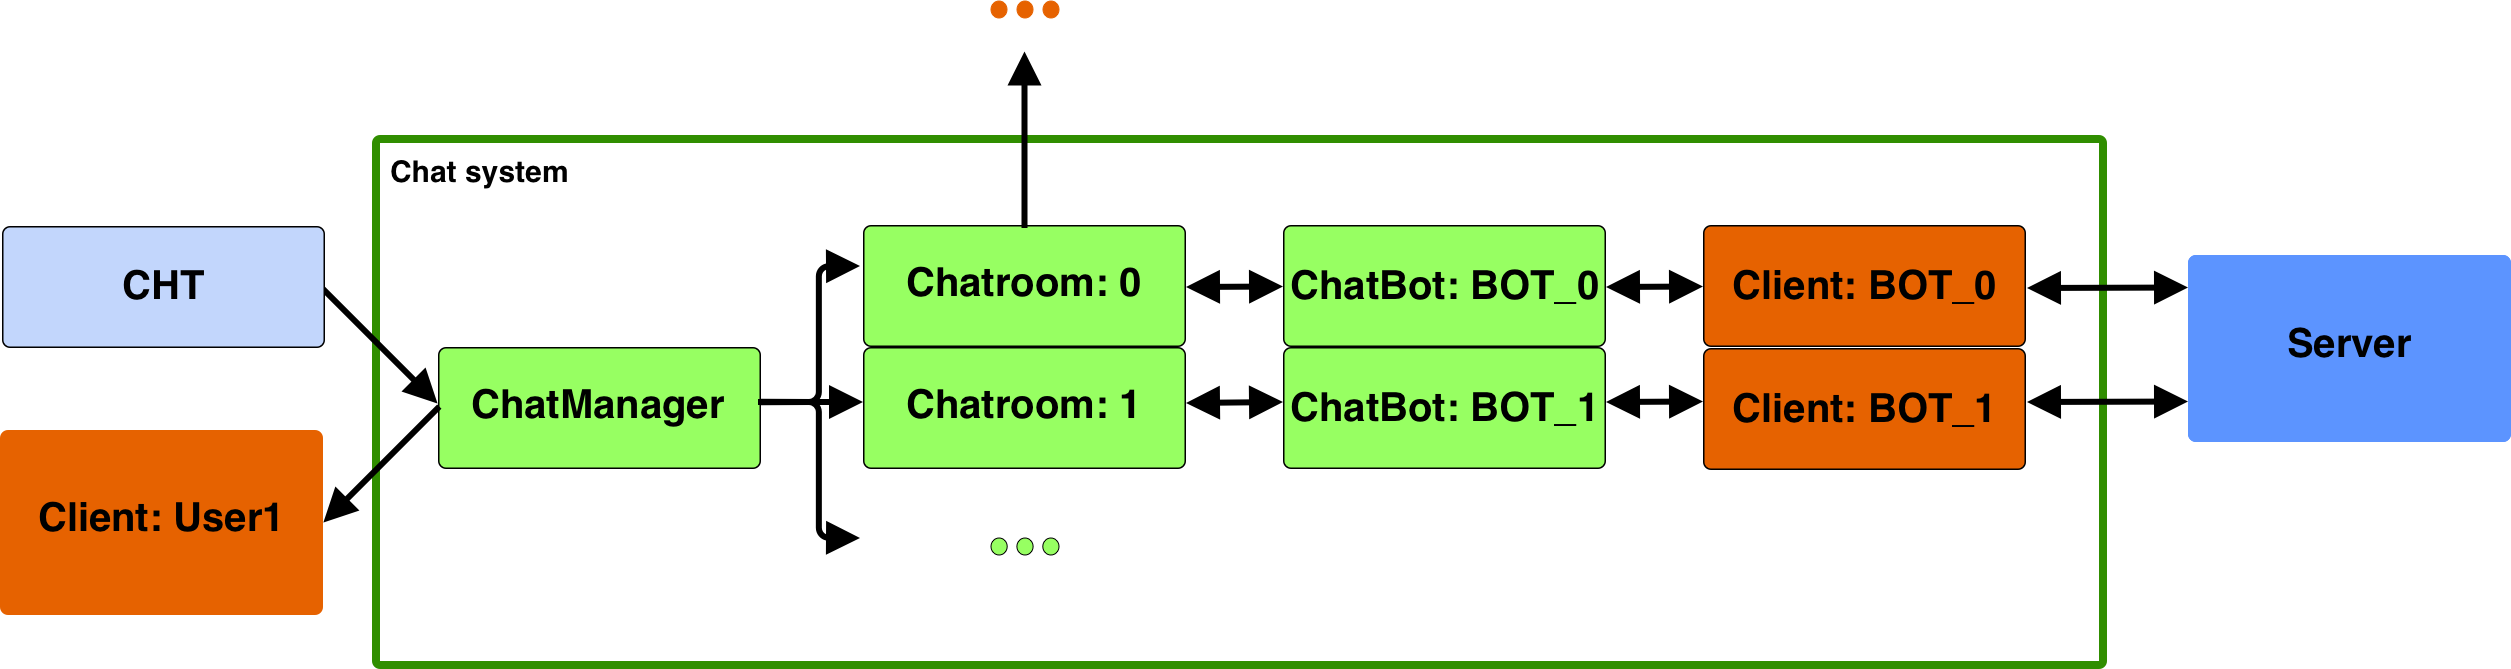
\includegraphics[width=\linewidth]{figures/chat/chat_arch.png}
	\caption{Client side architecture}
\end{figure}

\begin{figure}[h]
	\centering
	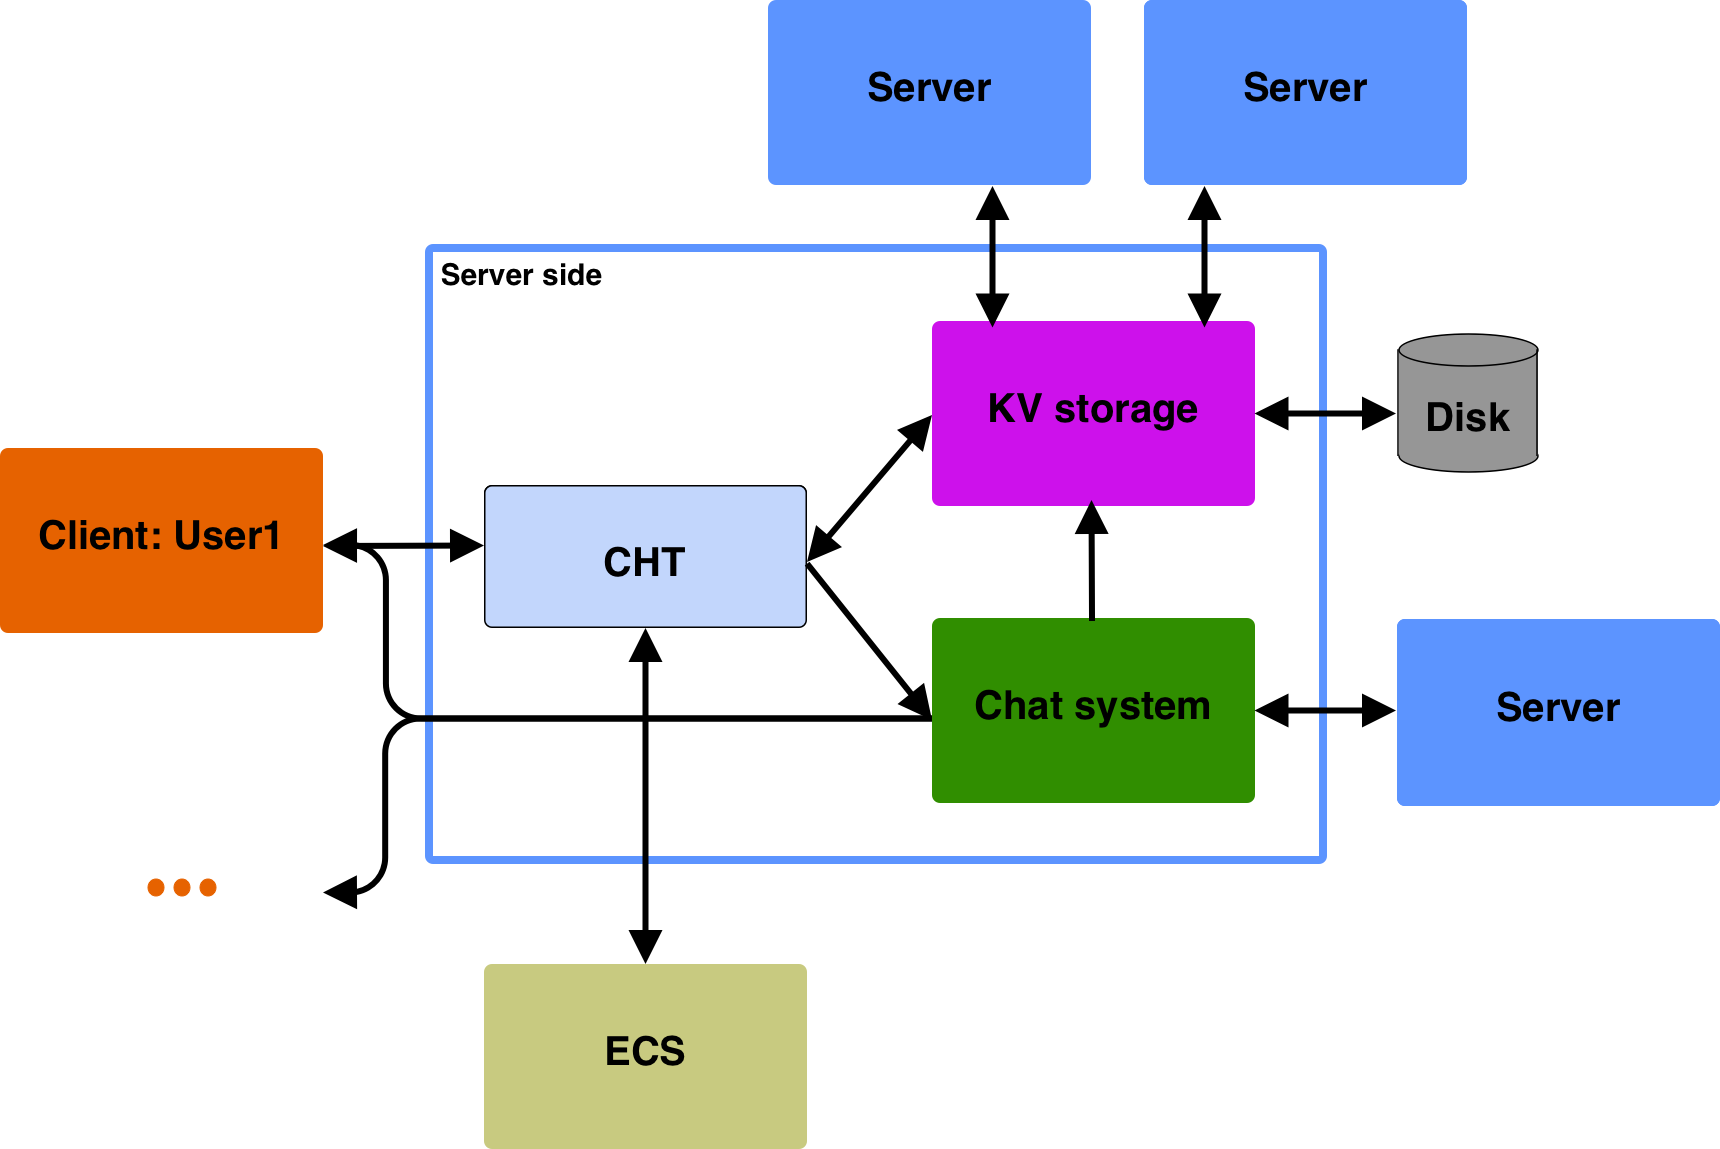
\includegraphics[width=\linewidth]{figures/chat/chat_full_arch.png}
	\caption{Client side architecture}
\end{figure}

chat system:
All chat related requests get transferred by the CHT to the ChatManager. This has a list of Chatroom objects. When a client tries to connect to a chatroom, the ChatManager checks the list whether a chatroom with the provided chatID already exists or not. In the former case, 
if the chatroom is public, the client is granted access or, in case of a private chatroom, requested to enter a password. In the event of no chatroom found with the given chatID, the client is allowed to create the chatroom by specifying its type and providing a password, if a private chatroom is chosen. In order to increase security, the password gets hashed on the client side and only the hash of the password is stored at the server side and used for validation.

